\documentclass[12pt, titlepage]{article}
\usepackage{listings}
\usepackage{parskip}
\usepackage[utf8]{inputenc}
\usepackage[spanish]{babel}
\usepackage[margin=2.5cm]{geometry}
\usepackage{setspace}
\onehalfspacing
\usepackage{graphicx}


\title{Reporte del proyecto 1}
\author{Figueroa Ramirez Jesus}
\date{\today}
\begin{document}

\maketitle

\newpage

\section{Introducción}
En este documento se presentará el proceso de desarrollo del primer proyecto de la clase de modelado y programación el cual corresponde a un Chat en terminal.

El proyecto consistía en dos partes, el desarrollo del servidor y del cliente los cuales son dos programas independientes que se comunican mediante un protocolo dado en la especificación del proyecto.

El servidor debía ser capaz de recibir mensajes correspondientes al protocolo mediante diccionarios de \lstinline|JSON| y procesar estas peticiones para responder de acorde al protocolo.

El cliente debía ser capaz de interpretar estos mensajes y mostrarlos en texto natural al usuario y recibir la entrada del mismo para procesarla y generar un mensaje correspondiente al protocolo con la instrucción necesaria para el servidor.

Las funciones especificadas son:
\begin{itemize}
	\item Mensajes públicos: Cualquier usuario del chat se debe encontrar en la sala general en la cual puede recibir mensajes de todos los usuarios conectados y así mismo puede enviar mensajes a todos los usuarios.
	\item Mensajes privados: Cualquier usuario conectado puede enviar y recibir mensajes privados de cualquier otro usuario.
	\item Notificación de conexión y desconexión: Los usuarios deben recibir una notificación cada que un usuario se conecta o desconecta.
	\item Grupos: Los usuarios deberían ser capases de crear grupos e invitar a cualquier usuario conectado.
	\item Notificación de grupos: Cada que un usuario de conectará o desconectará de un grupo, los usuarios del mismo deben de ser notificados.
\end{itemize}

\section{Desarrollo}
\subsection{Análisis}
El inicio cualquier proyecto parte por en análisis de aquello que queremos lograr para así poder plantear una solución adecuada, en este caso el una lisis correspondía a entender adecuadamente la especificación y plantear un modelo de solución.

En este caso la primer observación fue que el servidor y cliente debían ser dos entidades totalmente separadas cuya única conexión sería mediante los diccionarios de \lstinline|JSON| ya que cada una debía existir por separado, ya que los usuarios no deberían tener acceso directamente al servidor.

Debido a la inexperiencia desarrollando proyectos desde cero la etapa del análisis no fue muy extensa ya que no comprendía adecuadamente el como debía ser la estructura del proyecto, debido a ello y a el limite de tiempo decidí que lo mejor era empezar a buscar las herramientas de desarrollo y empezar con el mismo lo antes posible para así tener margen para que al inevitablemente cometer errores poder solucionarlos en tiempo y forma.

El siguiente paso fue seleccionar el lenguaje de programación que utilizaría, en este caso mi primer pensamiento fue utilizar java ya que era el lenguaje en el que más experiencia tenía en el momento, sin embargo esta idea rápidamente fue desechada ya que dentro de la especificación del proyecto se mencionaba que utilizar java restaría un punto a la calificación del proyecto, por ello empece a considerar otras opciones, durante la especificación también se mencionó que el utilizar ciertos lenguajes podía ganar un punto extra en la calificación y entre estos lenguajes estaba \lstinline|Rust|, antes había escuchado de este lenguaje ya que se mencionaba que en los últimos años era de los lenguajes de programación con los que los desarrolladores se sentían mas satisfechos al programar, además de que se mencionaba constantemente que era un lenguaje de programación con un rendimiento muy bueno y que cada vez era más adoptado en el mundo del desarrollo, por último se hablaba mucho de su compilador el cual era muy sensible a los errores lo cual provoca que se detecten muchos errores en tiempo de compilación y al lidiar con estos errores se reducen en gran cantidad los errores que puede haber en tiempo de ejecución los cuales en mi consideración son más complicados de arreglar, por todo ello decidí utilizar este lenguaje para el proyecto ya que además me parecía un reto interesante.

Una vez decidido el lenguaje de desarrollo empecé a sumergirme en el mundo de Rust con el libro oficial del lenguaje el cual me resulto muy útil para aprender lo básico del lenguaje, seguido de esto continué con la investigación de las bibliotecas que utilizaría para el proyecto, la primera fue la biblioteca para poder serializar y deserializar los diccionarios de \lstinline|JSON| en estructuras y estas mismas usarlas para generar diccionarios, encontré múltiples herramientas para esto sin embargo dada mi investigación encontré que la más utilizada y adoptada era \lstinline|serde_json| la cual tenía todas las funciones que yo necesitaba para este proyecto.

En el libro de introducción a \lstinline|Rust| se presentaban dos herramientas para manejar la concurrencia, la primera era nativa del sistema, los hilos de ejecución, sin embargo se mencionaba que para rust cada hilo de ejecución correspondía directamente a un hilo de sistema lo cual los hacía bastante potentes sin embargo para manejar peticiones simples tal vez no era lo adecuado ya que no se requería tanta capacidad de procesamiento, la segunda herramienta que se presentaba era \lstinline|Tokio| una biblioteca externa que manejaba la concurrencia de forma asíncrona, me pareció que esta era la herramienta adecuada ya que al tener taras asíncronas lo que sucede es que por ejemplo al leer de red puede ser que la red sea lenta o simplemente no haya nada que leer y lo que hace \lstinline|Tokio| es no bloquear la ejecución de otros hilos sino que espera a un futuro, es decir solo requiere recursos de sistema cuando la tarea puede ser realizada isa liberando recursos del sistema para que se ejecuten otras acciones, además cada tarea de \lstinline|Tokio| es extremadamente ligera ya que esta planeada para manejar una gran cantidad de acciones que no requieran mucha capacidad de procesamiento, algo que encaja perfectamente con el proyecto de chat, por ello decidí utilizar esta herramienta para el desarrollo.

Después de definir las herramientas a utilizar era hora de iniciar el desarrollo, dentro del análisis había llegado a la conclusión de que la parte del servidor era la más compleja ya que tenía que manejar múltiples clientes, así que decidí iniciar por el servidor.

\subsection{Etapa de desarrollo}
Comencé el desarrollo definiendo un módulo y una estructura para el servidor, esta inicialmente tenía un mapa para guardar los usuarios, una dirección ip, un puerto y una variable para guardar el número de usuarios.

Una vez definida esta me quedaba claro que debía declarar otra estructura para los usuarios, la primer definición incluía como propiedades un socket, un nombre y el estado, para el estado decidí definir una enumeración para los tres estados posibles, también definí un método constructor para los usuarios que tomaba como parámetros el socket, el nombre y establecía por defecto el estado en Activo.

Teniendo en cuenta el protocolo el siguiente paso lógico era definir una estructura que me permitiera instanciar los mensajes que podía enviar el servidor, la decisión más lógica a mi punto de vista era una enumeración aprovechando las propiedades de las enumeraciones en Rust que permiten añadir parámetros los cuales asociaría a los distintos parámetros que recibían los mensajes en le protocolo.

Una vez con esto el siguiente paso era generar un método para instanciar un servidor, de hecho fueron tres, uno que recibía la dirección ip y el puerto, otro que establecía una dirección y puerto por defecto y un tercero que establecía la conexión en el localhost con propósito de los test, el siguiente paso fue definir un método para correr el servidor, este recibía un servidor envuelto en \lstinline|Arc<Mutex<>>|, \lstinline|Arc| era necesario pues así se podían enviar clones del servidor a múltiples funciones y que se compartiera el estado, por otra parte \lstinline|Mutex| permitía modificar las propiedades del servidor sin tener problemas de concurrencia. En la función run se llamaba a otra función auxiliar que se encargaba de recibir conexiones del servidor, esta función tomaba cada conexión y lo enviaba a una función que se encargaba de procesar la identificación inicial.

Esta función tomaba el socket y lo partía en dos, una parte para lectura y otra para escritura, después se encargaba de recibir el primer mensaje de el cliente el cual se serializaba a la instancia correspondiente y en caso de error mandaba el mensaje correspondiente al protocolo y desconectaba al usuario, si el mensaje era el correspondiente verificaba si el nombre ya existía y en ese caso llamaba a una función auxiliar para reintentar la identificación, en caso de una identificación exitosa se instanciaba un nuevo usuario con los sockets generados y el nombre proporcionado por el usuario, este mismo usuario se insertaba en el mapa de usuarios usando como clave su nombre.

Esta versión del servidor tenía varios problemas, el primero era que para insertar a un usuario se debía bloquear el servidor lo cual llevaba a mucho código repetido además de que podía llevar a que el servidor se alentara pues cada que se insertaba el usuario este se bloqueaba para cualquier otra operación, el segundo era un problema de carrera, al guardar los sockets en el usuario directamente, sobre todo para el socket de escritura llevaba a un problema grave,si la intención era manejar un mensaje para después enviar la respuesta accediendo al socket y escribiendo en él, nada evitaba que dos tareas intentaran hacer esto simultáneamente lo cual podía llevar a la corrupción de los mensajes en el mejor de los casos o a que todo el programa crasheara, entonces me quedaba claro que la única forma era que una única tarea pudiera escribir en el socket eliminando la posibilidad de errores en ese aspecto.

Investigando como podía resolver estos problemas me encontré con dos herramientas, la primera era una biblioteca llamada \lstinline|DashLine| este era un mapa seguro bajo las operaciones de concurrencia y que no necesitaba de una referencia mutable para modificarlo, lo que hacía el uso de \lstinline|Mutex| innecesario y permitiendo agilizar las operaciones en el servidor, con esta herramienta el código paso a ser mas legible y simple, por otra parte encontré que \lstinline|Tokio| tenía una herramienta llamada canales de comunicación, estos canales tenían un costo muy bajo de procesamiento al clonarse y por tanto permitían una comunicación efectiva entre las tareas.

Implementando los canales ahora al guardar un usuario no se guardaba sus respectivos sockets de lectura y escritura sino que se guardaba únicamente su comunicador, por el se enviaban los mensajes que el usuario iba a recibir y en una única tarea de \lstinline|Tokio| se encontraba el socket de escritura que se encargaba de tomar cada mensaje en el receptor y enviarlo al cliente correspondiente, así evitando los problemas de múltiples tareas tratando de escribir al mismo tiempo, siguiendo la misma filosofía ahora se generaba una única tarea para leer del socket del usuario y enviar los mensajes a procesar.

Al revisar el protocolo y los mensajes surgía otro problema, los mensajes que recibía el servidor no contenían ninguna información de quien los enviaba, esto hacía que con el diseño actual no se tuviera ninguna información de a quien responder los mensajes o información de quien los enviaba para generar los mensajes al resto de usuarios.

Pensando en una solución para esto pensé en una carta, una carta tiene un destinatario, un remitente, la fecha y el lugar del que se envía y el mensaje correspondiente, entonces ¿por que no generar cartas? Entonces definí una estructura llamada letter que tenia como propiedades el nombre del usuario que la enviaba, una dirección a la que responder que en este caso era el comunicador que enviaba mensajes a la tarea encargada de enviar los mensajes al usuario y por último el mensaje que había enviado, ahora al generar la función que recibía mensajes del usuario se pasaba un clon del comunicador y el nombre del usuario para así poder adjuntarlos a la carta al recibir un mensaje y enviar la misma a procesar.

Aún no hemos hablado de como procesar la cartas, en principio pensé en agregar una propiedad al servidor que sería una Cola de mensajes para que el método encargado de procesar los mensajes los obtuviera de esta cola, sin embargo esto nos llevaba de vuelta a \lstinline|Mutex| así que deseché esta idea para después notar que el receptor de la función que enviaba mensajes al usuario en realidad funcionaba como una cola, los mensajes se almacenaban en el receptor y la tarea encargada de enviarlos extraía uno a la vez para enviarlo, entonces ¿Por que no usar esto para procesar las cartas? Entonces agregue un canal de comunicación global, cada tarea encargada de recibir mensajes del usuario tenía una copia del comunicador para enviar cartas a procesar y una tarea se encargaba de procesar cada una de ellas.

Por último faltaba la implementación de los cuartos, lo primero fue definir la estructura encargada de modelar los cuartos de nombre Room, tenía 3 propiedades, un mapa de usuarios, un mapa de invitados y un nombre, con estas propiedades era suficiente para que los cuartos pudieran manejar las invitaciones y los menajes del cuarto, sin embargo había un pequeño problema con la desconexión de un usuario, cuando un usuario se desconectaba había que eliminarlo de todos los cuartos en los que estaba pero también eliminar las invitaciones ya que en caso de no hacerlo se podría conectar otro usuario con el mismo nombre y acceder a cuartos a los que no fue invitado, era posible solucionar esto recorriendo todos los grupos sin embargo no era lo ideal ya que al tener que recorrer cada elemento del mapa de cuartos debíamos bloquear una parte del mapa para evitar problemas de concurrencia, entonces cada que un usuario se desconectara el mapa de cuartos quedaría parcialmente bloqueado para operaciones de otros clientes, por ello y para reducir el número de operaciones que se llevaban a cabo se decidió implementar una mapa de cuartos en los que un usuario estaba y un mapa de cuartos a los que estaba invitado, en la estructura de usuario, evitando así recorrer todos los grupos del servidor de manera innecesaria cada que había una desconexión.

Lo último de la implementación del servidor fue re factorizar el código para que cumpliera mejor con el paradigma de programación orientada a objetos, en este caso sobre todo modificar las funciones del servidor para estar asociadas a un objeto del tipo servidor en lugar de ser funciones que recibían como parámetro un objeto del tipo servidor.

El desarrollo del cliente fue mucho mas simple, ya que una vez teniendo los mensajes que recibe y que envía el servidor son idénticos excepto que con función inversa, el cliente recibe los mensajes que envía el servidor y envía los que el servidor recibe, teniendo esto en cuenta se definen las enumeraciones para manejar los mensajes del servidor y para generar los mensajes a enviar, el manejo de los mensajes del servidor es muy sencillo ya que solo se debe imprimir el mensaje correspondiente para que el cliente pueda responder al mismo.

Se define un lenguaje de comandos para poder decir la acción que se quiere realizar, en este caso usamos /comando parámetro1 parámetro2, hay ciertos casos en los que no se recibe ningún parámetro en cuyo caso se ignoran si es que el usuario lo da, en caso de ejecutar un comando con menos parámetros que los requeridos, no se realiza ninguna acción y se envía el mensaje de ayuda con la especificación de todos los comandos y los parámetros que reciben, en el controlador simplemente se observa el comando y se utilizan los parámetros para generar el mensaje correspondiente para el servidor.
\section{Conclusiones}
Podemos observar en la figura \ref{fig:arquitectura} la estructura final de módulos del servidor, así mismo en la figura \ref{fig:arquitectura_cliente} la estructura final de módulos del cliente.

\begin{figure}
	\centering
	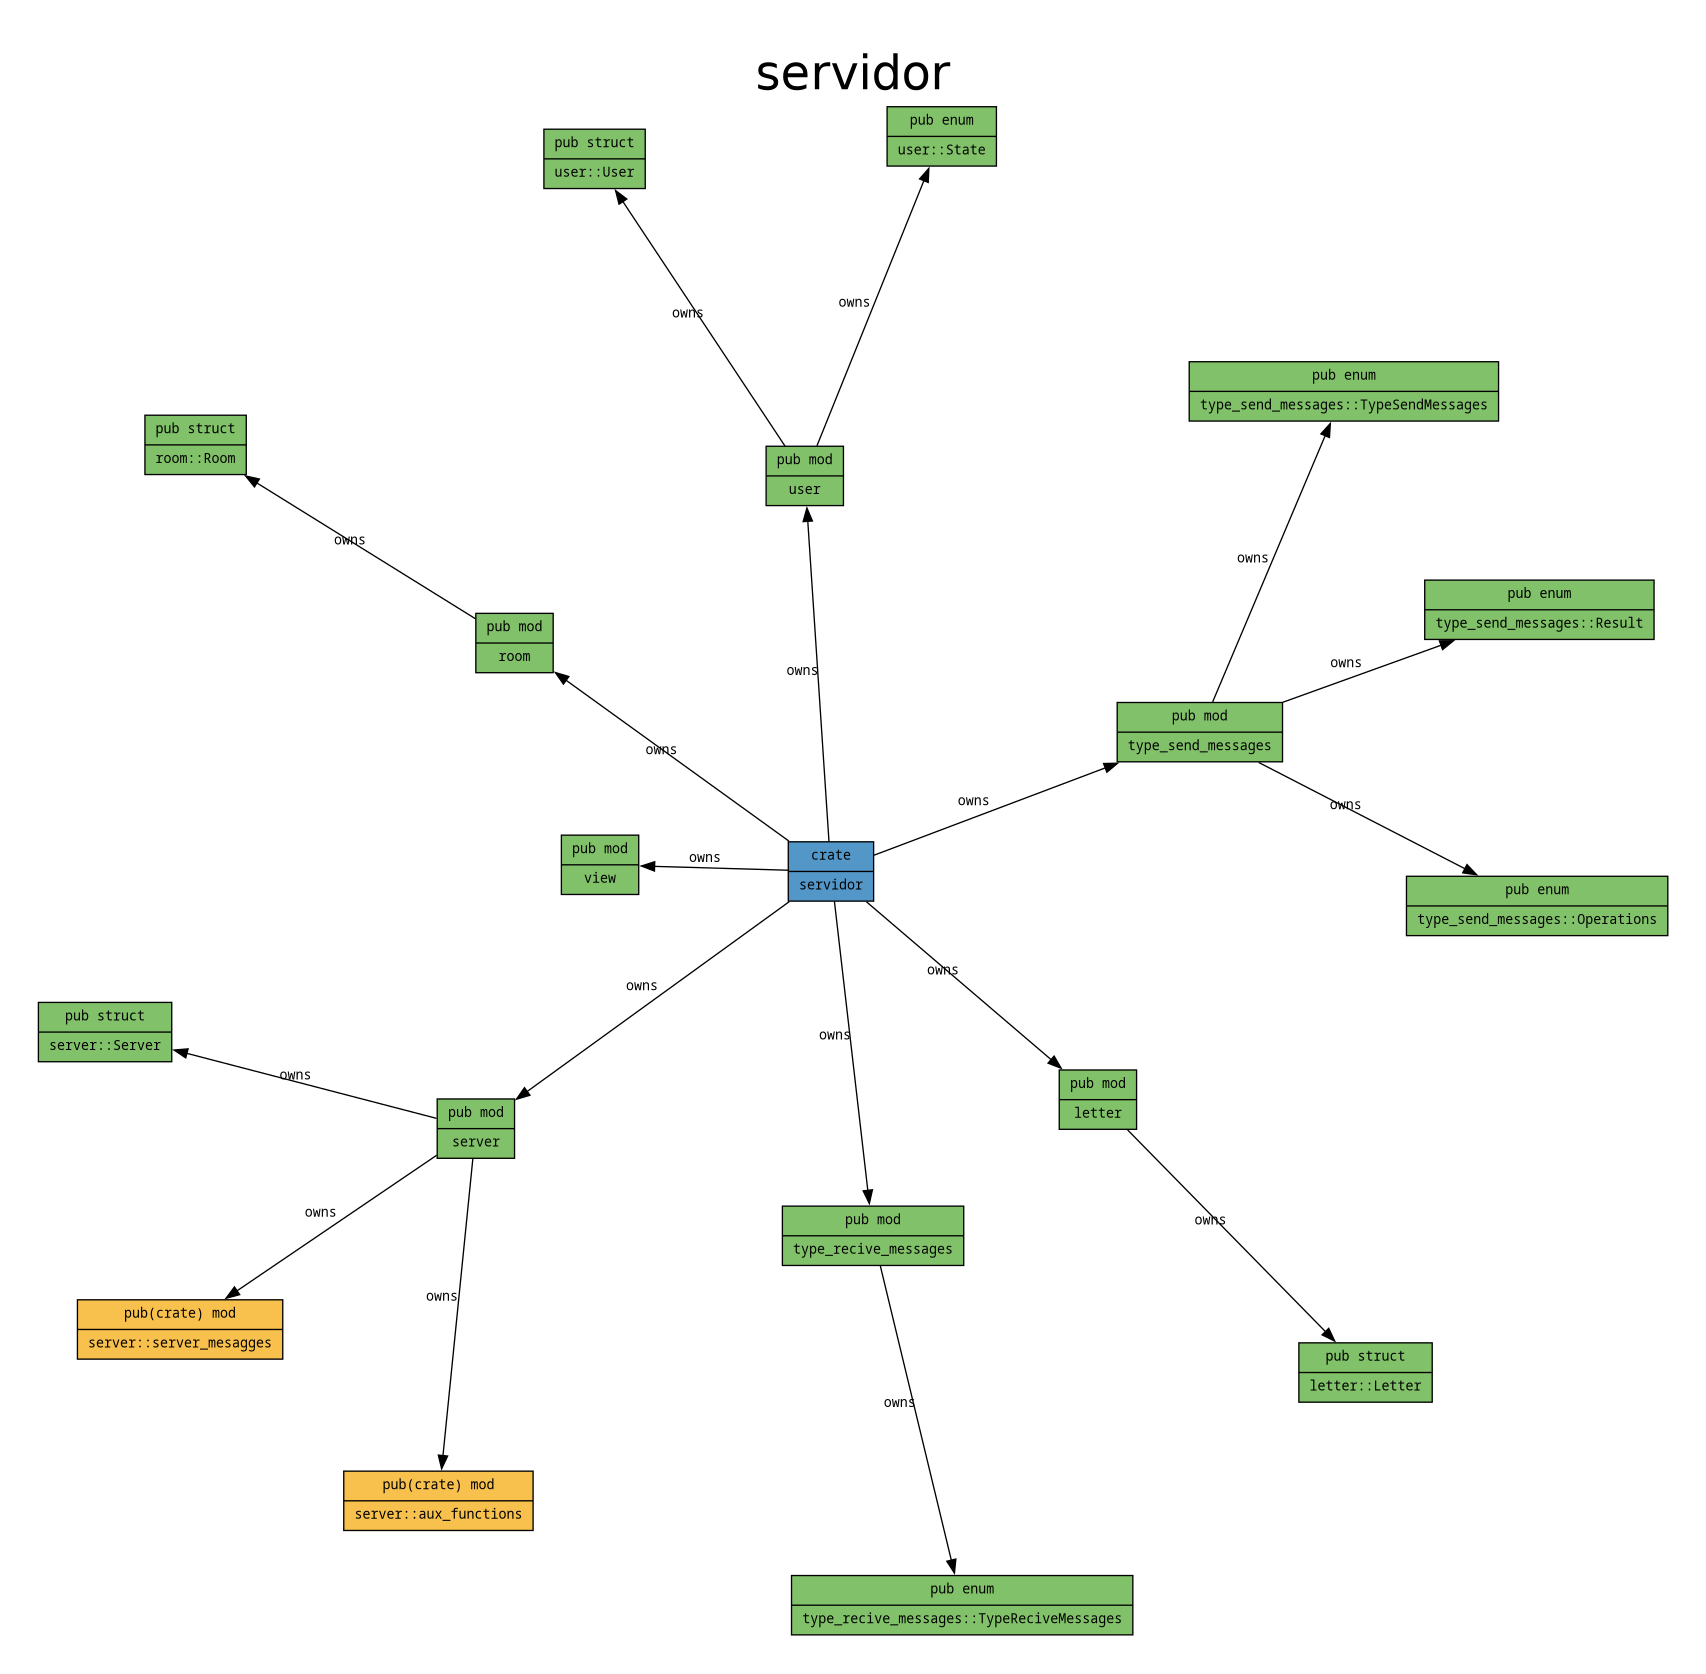
\includegraphics[width=0.8\textwidth]{estructura_servidor.png}
	\caption{Diagrama de módulos y estructuras del servidor.}
	\label{fig:arquitectura}
\end{figure}

\begin{figure}
	\centering
	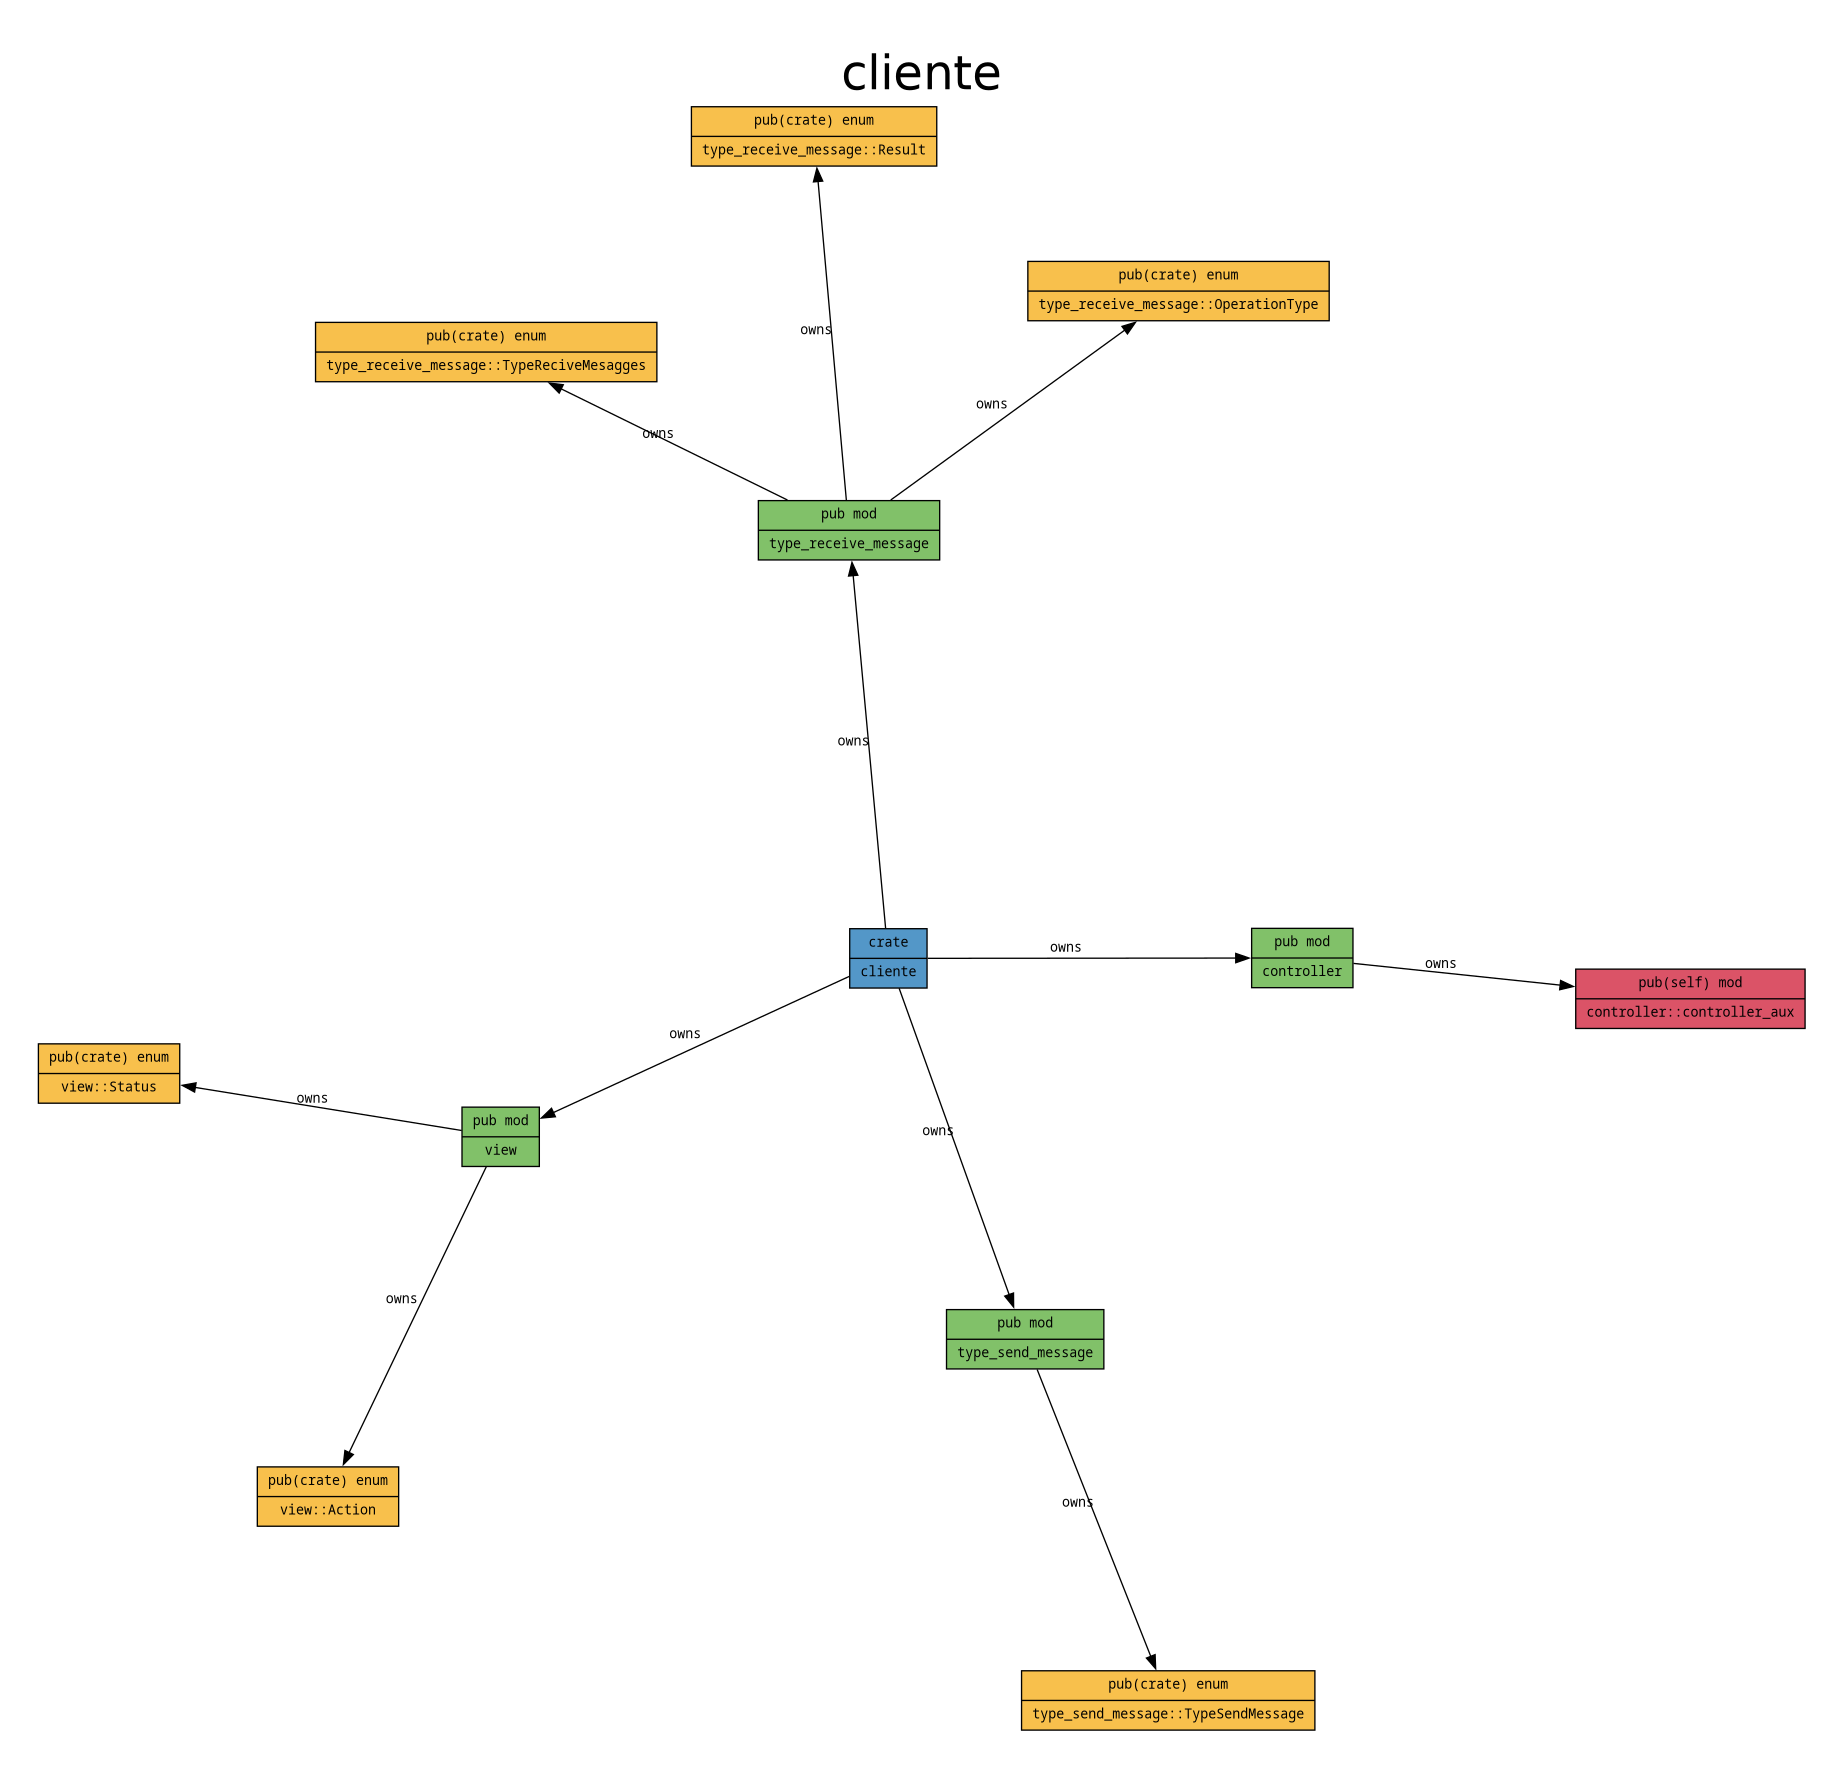
\includegraphics[width=0.8\textwidth]{estructura_cliente.png}
	\caption{Diagrama de módulos y estructuras del cliente.}
	\label{fig:arquitectura_cliente}
\end{figure}
\newpage
Durante la prueba de estrés llevada a cabo en la clase el servidor fallaba ya que no contestaba a ningún mensaje enviado por la prueba, esto me llevo a pensar en que podría estar sucediendo, mi teoría era que la prueba del profesor no enviaba un salto de línea para cada mensaje lo que provocaba que el servidor nunca leyera los mismos ya que en el diseño el servidor leía hasta un salto de linea y como no recibía este salto, jamás contestaba el  mensaje, entonces ese día cree una prueba de estrés que identificara a 50 clientes con una separación de 10 milisegundos cada uno y a la hora de correr el servidor contestaba adecuadamente a todos ellos, después añadí que cada uno de ellos enviara un mensaje público y después solicitara la lista de usuarios, prueba que también resulto exitosa, además el tiempo de procesamiento de todos los mensajes era menor a 1000 milisegundos lo cual era bastante razonable para la cantidad de mensajes que se manejaban.

Teniendo en cuenta todo lo anterior me atrevo a decir que las decisiones de diseño fueron las adecuadas pues el servidor funcionaba adecuadamente e implementaba todas las funcionalidades requeridas.

\end{document}
